% 图 6.21 两支自旋箭头夹角 theta 示意
\documentclass[tikz,border=5pt]{standalone}
\usetikzlibrary{arrows.meta}
\usepackage{amsmath}
\usepackage{bm}
\usepackage{fontspec}
\setmainfont{Times New Roman}
\begin{document}
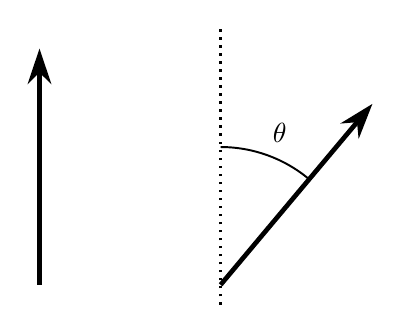
\begin{tikzpicture}[line width=0.8pt,>=Stealth]
% left spin (vertical)
\draw[->,line width=1.7pt,>={Stealth[length=4.5mm,width=3mm]}] (0,0) -- (0,3);
% right spin, deflected by theta (about 40 deg) from vertical
\coordinate (R) at (2.3,0);
\draw[->,line width=1.7pt,>={Stealth[length=4.5mm,width=3mm]}] (R) -- ++(50:3);
% dotted reference line (vertical) through right spin
\draw[dotted,line width=0.9pt] (2.3,-0.25) -- (2.3,3.25);
% angle arc
\draw[line width=0.7pt] (2.3,1.75) arc[start angle=90,end angle=50,radius=1.75];
\node at (3.05,1.93) {$\theta$};
\end{tikzpicture}
\end{document}
